\section{User Interface}
The user interface (UI) is perhaps one of the most important aspects of Fidelis; the UI dictates how users interact with the system, and serves as the single point of entry for user data. Fidelis needs to be able to engage the audience from the moment they land on the homepage and encourage the users to explore further by providing an easy to use and intuitive UI. This can be achieved by following standards defined by several committees and adhering to good practices. In addition to the engagement the Fidelis UI must also be usable and simple whilst remaining elegant and intuitive. Responsive design is also crucial to provide access to the system across a range of devices, and this is discussed later in more detail. The provided designs were produced as mock-ups, but were designed in such a way as to closely replicate the final product.

\subsection{Sitemap}
Figure \ref{fig:sitemap} shows the sitemap for Fidelis. This signifies the navigation routes the user will be able to follow on the site. Both sets of users (authorised and authorised) will be able to visit:
\begin{itemize}
\item Discover page - The Discover page will contain posts from a number of categories
\item Profile page - The Profile page will include details on a specific user, including the number of posts they have made and the posts they have voted on
\item Privacy page - The Privacy page will provide details on the Fidelis Privacy policy
\item Support page - The Support page will provide general support to users, such as Frequency Asked Questions (FAQs)
\end{itemize}

However, the Home page, which will contain a feed of posts followed by an authorised user, and the Settings page will only be accessible to authorised users.

\begin{figure}
\centering
\includegraphics[height=2.7in]{Images/Design/sitemap}
\caption{Fidelis Sitemap}
\label{fig:sitemap}
\end{figure}

\subsection{Navigation}
A navigation bar provides users with a quick way of accessing pages on a website. The navigation is usually located at the top of the page, and includes `quick-link' icons that enable the user to easily navigate to pages represented by the icon. Figure \ref{fig:navs} shows the navigation bars for Facebook and Twitter. In both we can see shared elements, such as the profile and home icons. In addition to the icons, the navigation bars also have search boxes. These search boxes enable users to explore content available on each site by providing keywords.

\begin{figure}[H]
\centering
\begin{subfigure}{1\linewidth}
	
\includegraphics[width=1\linewidth]{Images/Design/fb-nav}
	\caption{}
	\label{fig:fb-nav}
\end{subfigure}
\begin{subfigure}{1\linewidth}
	
\includegraphics[width=1\linewidth]{Images/Design/twitter-nav}
	\caption{}
	\label{fig:twitter-nav}
\end{subfigure}
\caption{Navigation bar designs for (a) Facebook and (b) Twitter}
\label{fig:navs}
\end{figure}

By studying existing navigation bar designs, concept designs for navigation on Fidelis were created. These designs can be seen in Figure \ref{fig:fidelis-navs}. There will be two navigation bars - one for unauthorised users and the other for authorised users. Both designs employ intuitive icons that will allow the user to identify the page they will be taken to when the icon is clicked on. To signify the page users are currently on, an orange underline will highlight the icon corresponding to the page the user has navigated to. In addition to this, the navigation bar will also include a search field which will allow the user to locate specific categories or users. The two navigation bars differ slightly in the pages they allow the user to navigate to. When a user is not logged in, they will be unable to view their notifications (signifed by the bell icon), or view their profile. However, they will still be able to view public posts in a category they search for, or view a public user profile.

\begin{figure}[H]
\centering
\begin{subfigure}{1\linewidth}
	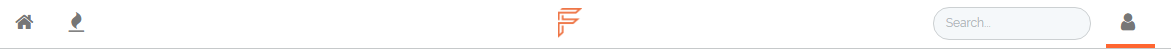
\includegraphics[width=1\linewidth]{Images/Design/nav-unauthorised}
	\caption{}
	\label{fig:nav-unauth}
\end{subfigure}
\begin{subfigure}{1\linewidth}
	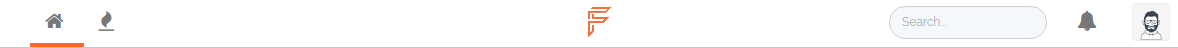
\includegraphics[width=1\linewidth]{Images/Design/nav-authorised}
	\caption{}
	\label{fig:nav-auth}
\end{subfigure}
\caption{Fidelis navigation bar designs for (a) unauthorised and (b) authorised users}
\label{fig:fidelis-navs}
\end{figure}

\subsection{Authentication}
User authentication involves either collecting the credentials of a user to verify their identity and retrieve the relevant data for that user, or allowing a user to register a new account. These two processes for authentication are normally represented with log-in and registration pages. The following sections will look at the design for each of these.

\subsubsection{Register}
The registration page should enable new users to enter their details and create an account on Fidelis. Sites vary in the details they collect during registration. Figure \ref{fig:reg-pages} shows the registration pages for Facebook, Twitter and Reddit. Each of the three sites collects user email addresses and passwords. These two pieces of information are constan across almost all registration pages, regardless of the website. In addition to this, Reddit, as seen in Figure \ref{fig:reddit-reg} asks only for a username. Twitter registration (Figure \ref{fig:twitter-reg}) does not require a username, and instead collect the users full name. Facebook registration collects even more user data, requiring a date of birth and gender in addition to what is already collected by Twitter. 

\begin{figure}
\centering
\begin{subfigure}[b]{.4\linewidth}
	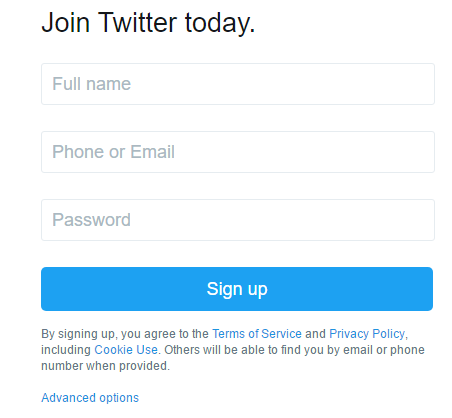
\includegraphics[height=1.5in]{Images/Design/twitter-reg}
	\caption{}
	\label{fig:twitter-reg}
\end{subfigure}
\begin{subfigure}[b]{.5\linewidth}
	\centering
	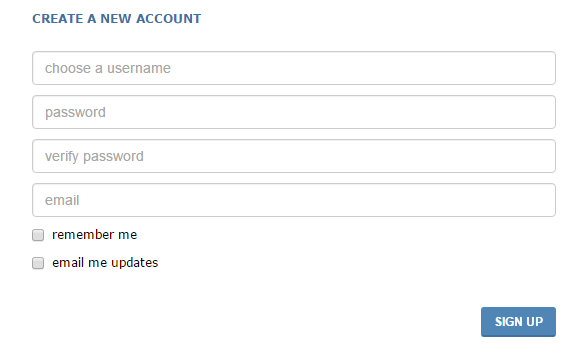
\includegraphics[height=1.5in]{Images/Design/reddit-reg}
	\caption{}
	\label{fig:reddit-reg}
\end{subfigure}
\caption{Registration pages for (a) Twitter and (b) Reddit}
\label{fig:reg-pages}
\end{figure}

Figure \ref{fig:register-page} shows the design for the Fidelis registration page. Users will be required to enter their name, email, username, date of birth and password. Although not entirely necessary initially, it was decided to retain user date of births as thought was put into future uses for it. As the system grows, it is inevitable that certain categories or tags will contain content unsuitable for younger audiences. Therefore, age can be used a tool to filter unsuitable content for younger users. In order to ensure that the user's are compliant with the terms of the site, they must mark that they agree to the terms of the site before registration can be completed.

\begin{figure}[H]
\centering
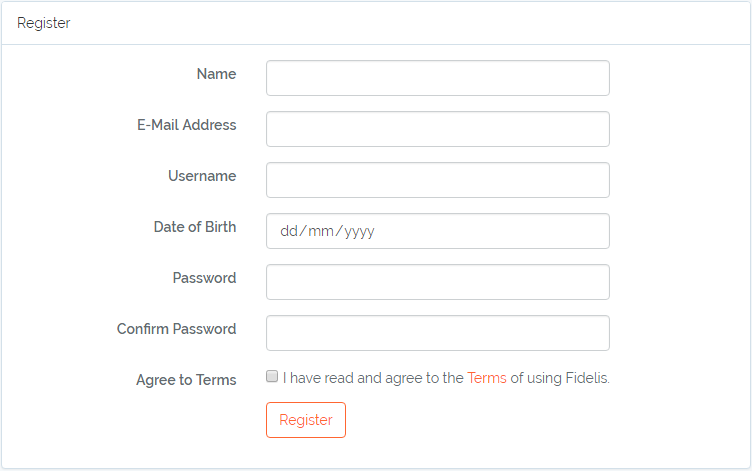
\includegraphics[height=2in]{Images/Design/register-page}
\caption{Design for registration page}
\label{fig:register-page}
\end{figure}

\subsubsection{Log In}
The log-in page should allow an existing user to enter their log-in credentials. On most sites this is a combination of either email or user name, and a password. To be able to correctly verify user identity, both email (or username) and password must be required fields. Users are responsible for remembering the log-in credentials, but are also liable to forget them. To prevent user accounts from being inaccessible, the log-in page should include a link that allows users to recover a forgotten password. A user may accidentally navigate to the log-in page, when they actually intended to navigate to the registration. As such, a link must exist on the log-in page which will take users to the registration page. Figure \ref{fig:login-page} shows the concept design for the log-in page, encapsulated all aforementioned aspects.

\begin{figure}[H]
\centering
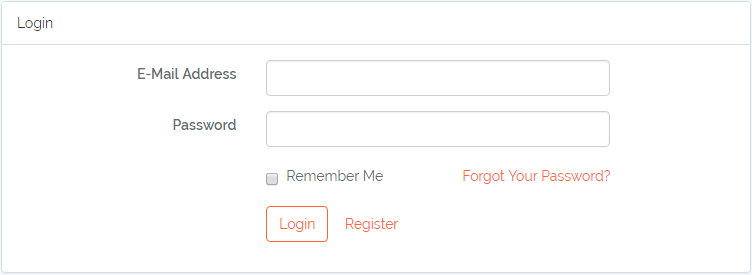
\includegraphics[height=1.5in]{Images/Design/login-page}
\caption{Design for log-in page}
\label{fig:login-page}
\end{figure}

\subsection{Home}
As with most websites, the home page is the central hub from which the user can navigate. This is often the first page that a user will see upon entering the website. Fidelis is no different in this regard. The Fidelis home is split into two different pages, one for when the user is logged in, another for when they aren't.

\subsubsection{Logged Out}
If a user is not logged in to the website, they will see a display shown in Figure \ref{fig:home_unauthorised}. This is the landing page for the site and will be the first port of call for any logged out users or users who are new to Fidelis. The background for this page is a full-screen image, randomly chosen from a select set of images. In the centre of the page there is the title Fidelis, as well as a quote relating to the core concept of the Fidelis platform: trust. Again, these quotes are chosen randomly from a set of quotes. The user can navigate using the buttons in the top right of the page to either log in or sign up for a new account.

\begin{figure}[H]
\centering
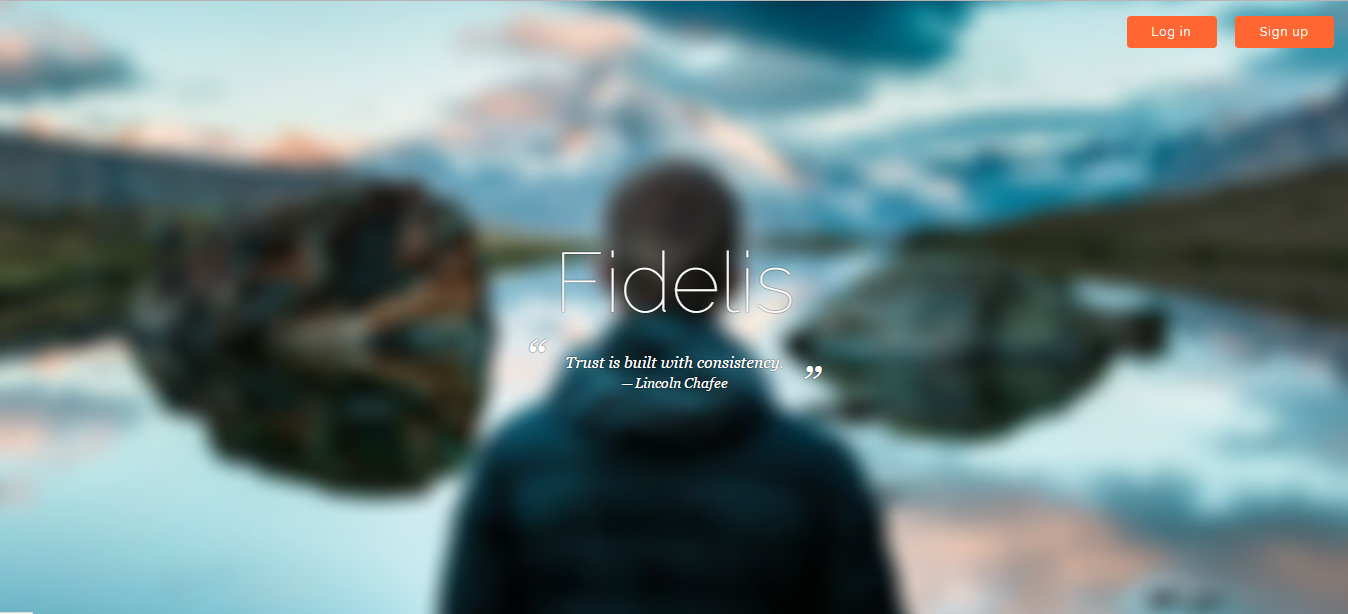
\includegraphics[width=\linewidth]{Images/Design/home_unauthorised}
\caption{Design for home page when not logged in}
\label{fig:home_unauthorised}
\end{figure}

\subsubsection{Home Page}
Once a user has logged in to their account, the will be directed to the home page, showing in Figure \ref{fig:home_authorised}. The page features the nav bar so the user can navigate to other pages, search for tags/users etc. The most prominent feature of this page is the central post feed. A user can create new posts including text and images as well as interacting with other posts. This includes upvoting or downvoting a post, commenting on a post and reporting posts. The posts displayed in this feed are selected by the system to match the user's interests.

When creating a post, a tagging system is used similar to Twitter which allows users to mention other users (using the @ symbol) and also to tag topics (using the \# symbol). These tag topics are used to create specific topic feeds in the discover page and to calculate the trending topics (see section \ref{sec:design-trending}). Any topic tags which exist in a post are added to the post\_tags table. In addition to tags allocated to a post using the \# symbol, tags are also added to a post if the post contains a word which already exists in the tags table. This allows for content which hasn't been explicitly tagged to be available in the discover page.

Other than the post feed there are a number of widgets the user can interact with. The user profile widget on the left shows information about the user. This widget links to the user's profile page as well as lists showing the user's posts, the user's followers or other accounts following the user. Also on the left of the page is a widget displaying suggestions for other accounts that the user can follow to expand their network. Again, these suggestions are bespoke for the current user. On the right side of the page is another widget showing the tags that are currently trending across the entire platform. This is another way that the user can find new content rather than seeing just the posts in their feed.

\begin{figure}[H]
\centering
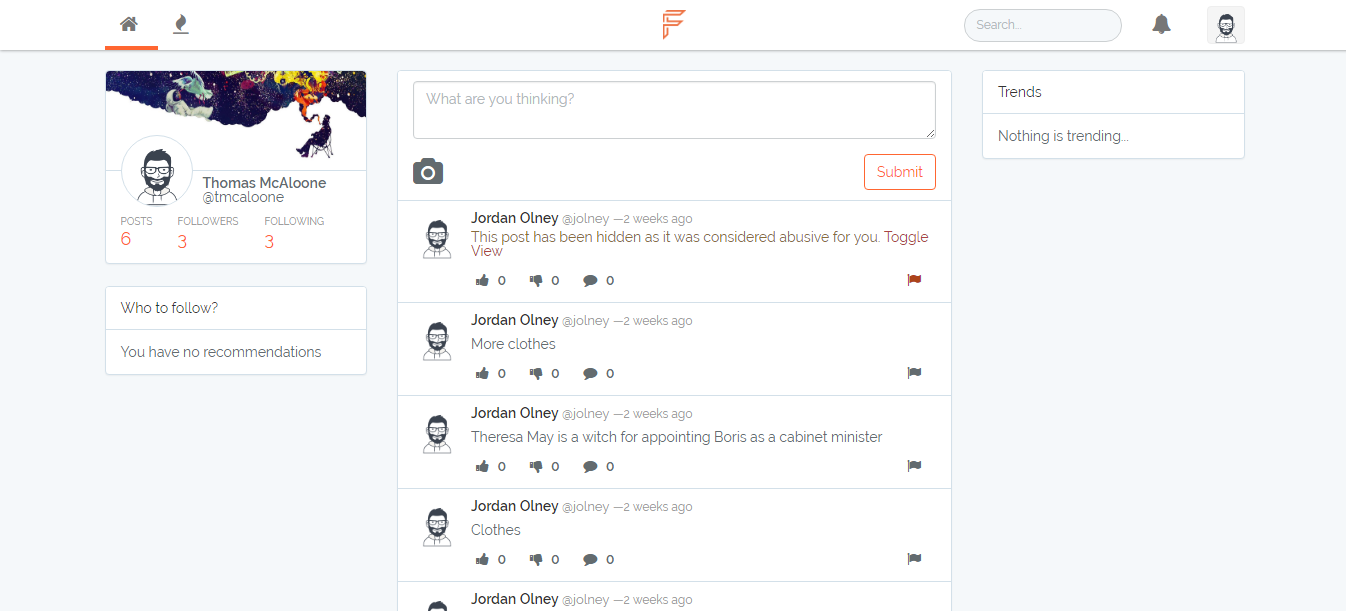
\includegraphics[width=\linewidth]{Images/Design/home_authorised}
\caption{Design for home page when logged in}
\label{fig:home_authorised}
\end{figure}

\subsection{Discover}
A major feature of the Fidelis platform is allowing users to seek out and find new content, which appeals to them, outside of their current network. The discover page allows this to happen. The page (Figure \ref{fig:discover_page}) shows a broad (albeit concise) list of categories which each have a number of tagged posts associated with them that the user can view and interact with.

\begin{figure}[H]
\centering
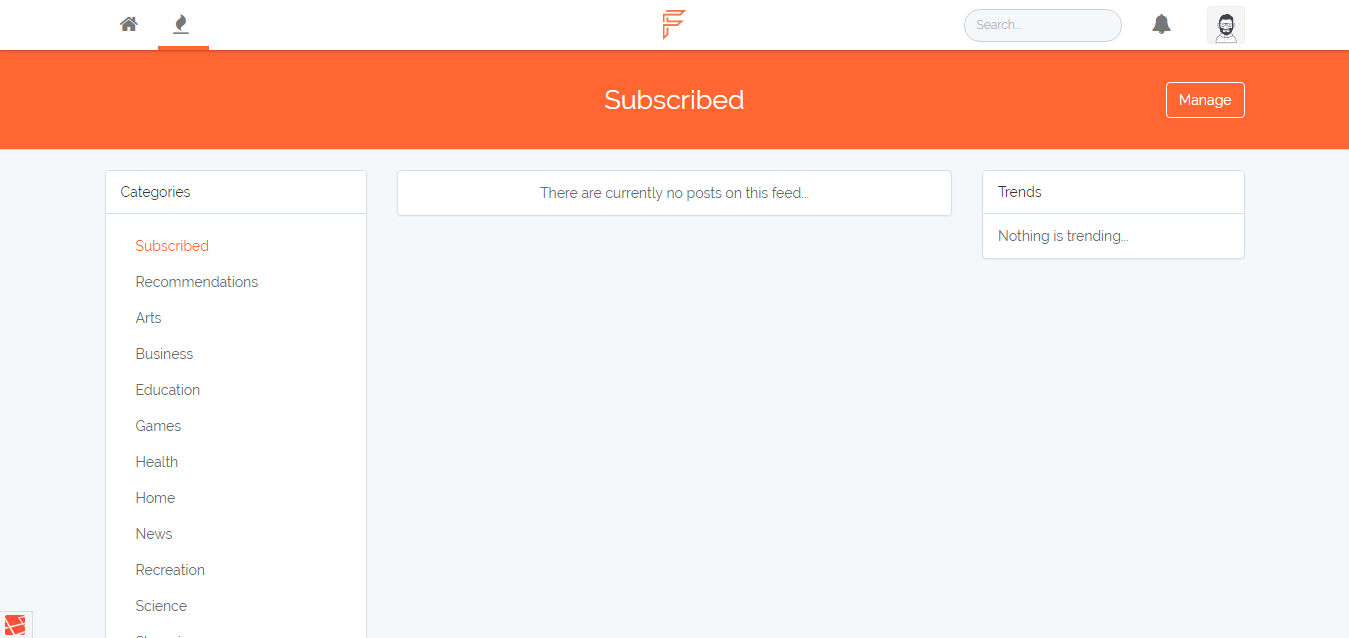
\includegraphics[width=\linewidth]{Images/Design/discover}
\caption{Design for discover page}
\label{fig:discover_page}
\end{figure}

On the left hand side of the page is a category list widget, displaying a list of categories which contain related posts. The user can select a category to see posts that fit with that category. This list also shows a `Subscribed' option, which when selected shows posts from topics the user is subscribed to. When a category is selected, the title of that category appears as a title across the top of the page. In the case of the `Subscribed' option, a `Manage' button is also shown here which links to the Settings page where the user can manage (add or remove) their subscriptions. In the centre of the page is the post feed, which in a similar manner to the post feed in the home page, shows a list of posts the user can interact with, however the posts shown will only be those that belong to the currently selected category. On the right hand of the screen is the trends widget which shows all of the tags which are currently trending across the entire Fidelis platform.

\subsection{Notifications}
Notifications are a key component to communication on social media platforms. Notifications give prompts to users on interactions that have occurred between them and other users. To let users know of a new interactions, notifications either give visual or auditory triggers that get a users attention. With the Google Chrome Notifiations API \cite{ChromeAPI:Notifications} it is now even possible to send notifications to user when they are not on the webpage itself. However, notifications on Fidelis will be provided using a number counter next to a bell icon, which will symbolise the notifications page. This is akin to the notification counter seen on most social media platforms. The page itself will contain a feed of notifications that will give information to the user on who the notification is from, and the type of notification it is. If the notification is a comment, it will include the comment from the user making it. If the notification is for a vote or a follow, it will only include information on the name of the user making the vote or follow. Figure \ref{fig:notifications-page} shows a mock-up of how the notifications page will appear. Here we can see a number counter next to the bell icon signifying the number of new notifications, and also a notification telling us that another user has commented on one of the posts we have made. In addition to the notifications themselves, the page will also include a profile widget, recommendations widget and trending widget. The user will be able to navigate to their profile from this page, and also interact with trending topics or new user recommendations.

\begin{figure}[H]
\centering
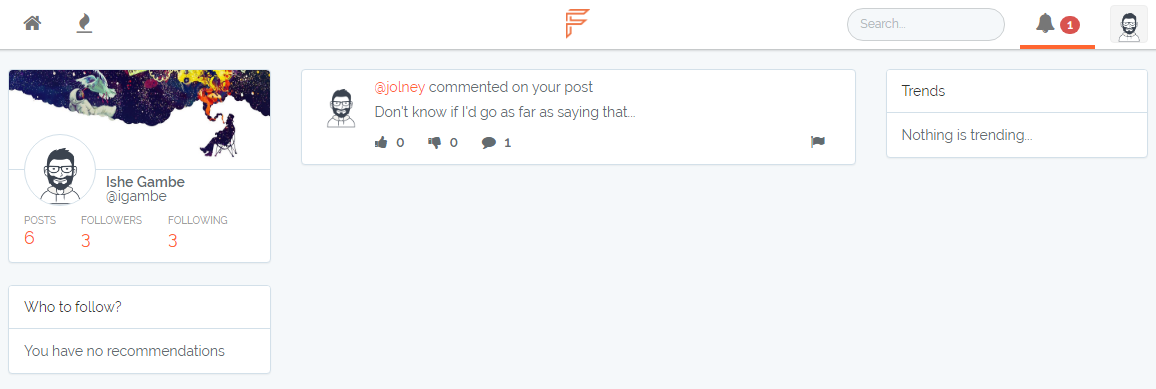
\includegraphics[width=1\linewidth]{Images/Design/notifications-page}
\caption{Design for Notifications page}
\label{fig:notifications-page}
\end{figure}

\subsection{Profile}
The user profile page (shown in figure \ref{fig:user_profile}) allows the user to see all of either their activity and public information related to their account (Name, bio etc.). The user can also view the profiles of other accounts which creates yet another avenue for discovering new content, as well as nurturing user-to-user interactions across the platform. Along the top of the page one can see the user's profile photo and cover photo, a feature allowing a user some expression to aid in building a personal presence on the platform. If the current page belongs to the user viewing it, the user is able to change their profile or cover photo by clicking the icon that appears when the cursor hovers over either image. Below the user's profile we can see some public personal information about the user. Here we also see a widget of photos that the user has uploaded. In the centre of the page we see a post feed displaying content the user can interact with. The content displayed is based upon which tab the user currently has selected. These tabs can be seen directly above the post feed. The posts tab will display all of the posts created by the account to whom the page belongs. The rated tab will display a history of all the posts that the account has rated (upvoted or downvoted). The follower and following tabs with display a list of all of the other accounts that this account follows, or is followed by respectively. The trending widget on the right of the page shows all of the tags currently trending across the platform. Finally there is a button on the right side of the page which changed depending on to whom the page belongs. If the current page is being viewed by its owner, the user will be given a prompt to edit their profile, in case there is any information they want to add, update or remove. If this current page is being viewed by someone who is not the user, the user will be given the opportunity to follow, unfollow or block the user who owns this page.

\begin{figure}[H]
\centering
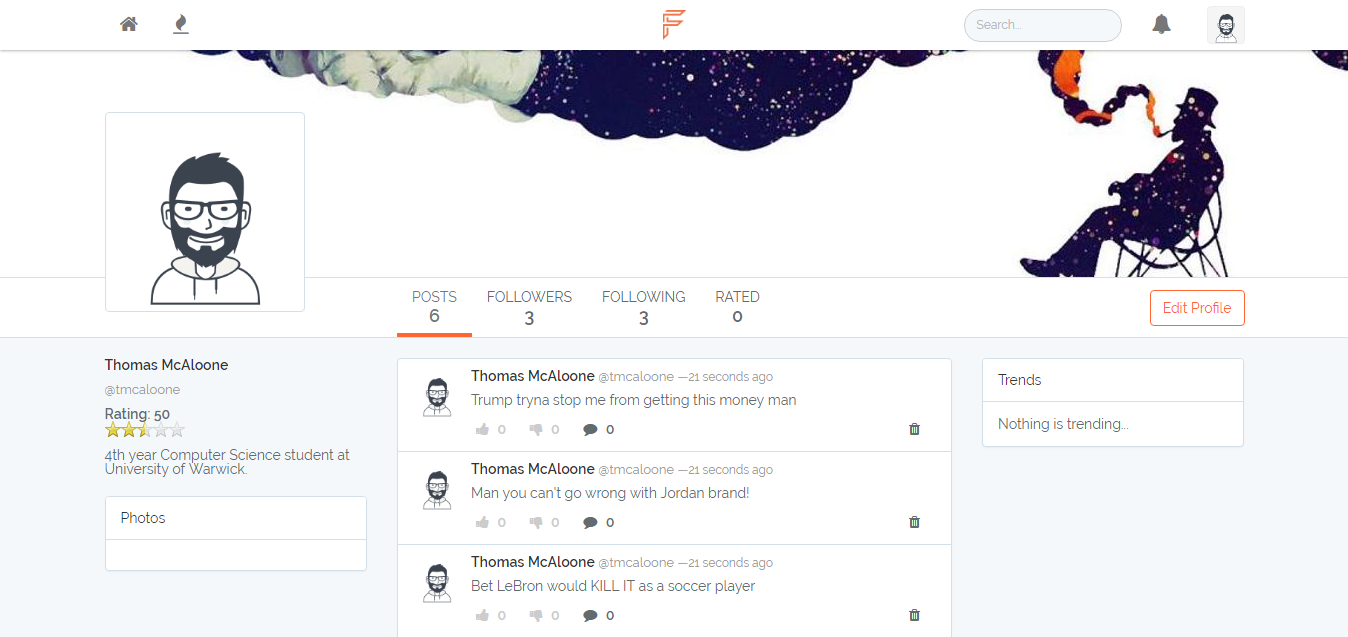
\includegraphics[width=\linewidth]{Images/Design/user_profile}
\caption{Design for user profile page}
\label{fig:user_profile}
\end{figure}

\subsection{Settings}
The settings page enables users to make changes to their user profile. It is important to provide users with the option to monitor and change their profile settings as they see fit. This gives them control over their account.  Settings generally included for user accounts include the ability to change their email address or update their passwords. Some websites, like Facebook and Google, allow users to control devices linked to the user account.

\begin{figure}[H]
\centering
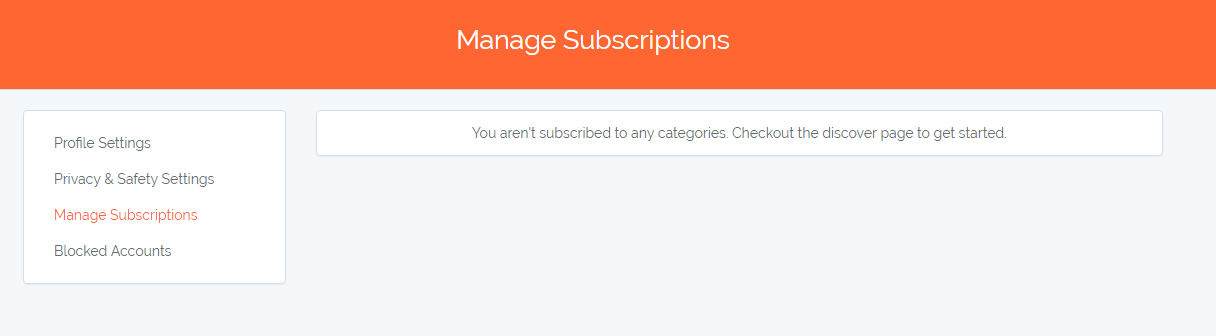
\includegraphics[height=1.5in]{Images/Design/SettingsPage}
\caption{Design for user settings page}
\label{fig:SettingsPage}
\end{figure}

Figure \ref{fig:SettingsPage} shows the design for the user settings page. Settings will be divided into: profile settings, privacy \& safety settings, tag subscription management and managing blocked accounts. Profile settings will allow the user to change their name or username, and toggle the privacy of their account. Privacy \& safety settings will provide users with a set of parameters used for data processing. The parameter values chosen by users will determine the outcome of data processing. An example parameter under the safety settings will be the reputation threshold that will be used during recommendation generation. The subscription management tab will allow users to view tags they are subscribed to, and unsubscribe from them if they no longer wish for their content to be shown in their subscribed feed. Finally, the blocked accounts tab will enable the user to view users they have blocked, and will provide the user with the option to unblock such users.

\subsection{Static Pages}
The two static pages aim to address the possible issues discussed in section \ref{Chapter:Issues}, by displaying information about the terms of use for Fidelis and providing support in order to help alleviate any personal issues which can arise through the use of social networking sites. These pages are accessible to both authorised users and guests visiting Fidelis. Both static pages are accessible via links in the footer of every page.

\subsubsection{Support}
The support page displays details of how to deal with content on the site which may distress the user. Fidelis aims to keep this content to a minimum, through the abuse detection, reputation scoring and terms of service, however, some content may still be posted on the platform which is not prevented via these measures. Therefore, the page lists options of how to remove the content, by reporting it and adjusting abuse detection settings. It also provides contact details to the Samaritans \cite{Samaritans:Home}, who can offer support in case of any social issues which may arise on the network such as cyber-bullying. As seen in figure \ref{fig:support}, the styling for the page is simplistic, using bullet points in order to break down the information being provided.

\begin{figure}[H]
\centering
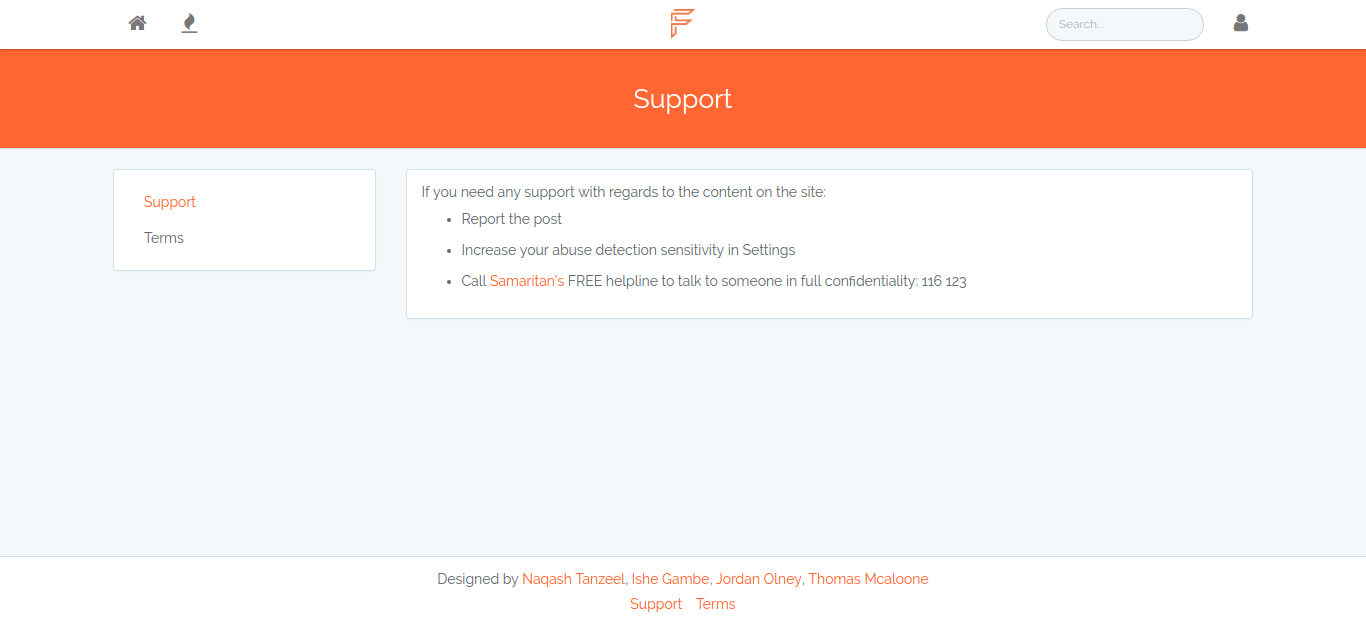
\includegraphics[height=2in]{Images/Design/support-page}
\caption{Design for support page}
\label{fig:support}
\end{figure}

\subsubsection{Terms}
The styling for the terms page is the same as the support page, using bullet points to make the information more readable, as shown in figure \ref{fig:terms}. However, the information provided is regarding the terms of service, to ensure that the user understands what is expected of them when using the site and the service Fidelis is expected to provide. This is to help avoid any legal issues which may arise from the content which is posted on the site by users.

\begin{figure}[H]
\centering
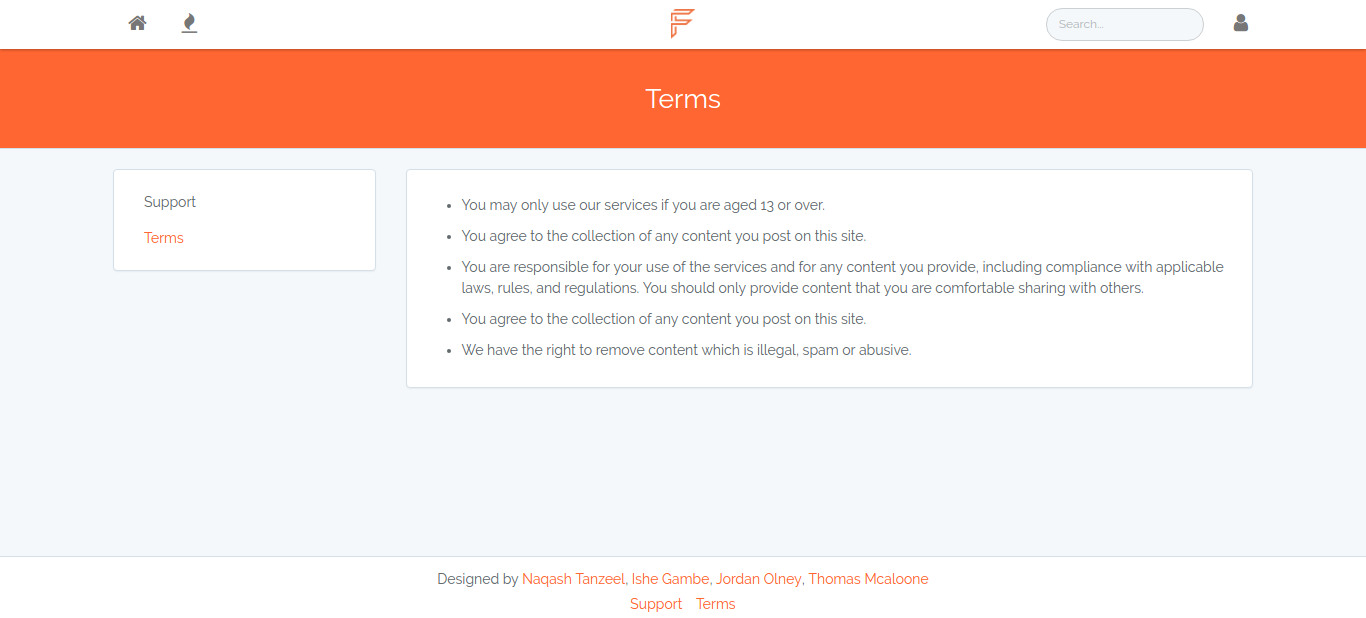
\includegraphics[height=2in]{Images/Design/terms-page}
\caption{Design for terms page}
\label{fig:terms}
\end{figure}

\subsection{Widgets}
Widgets are re-usable ``miniature application views'' that provide specified, limited functionality \cite{AndroidDevelopers:Widgets}. Widgets are extremely popular on mobile devices; in figure \ref{fig:WeatherWidget} we can see a widget for the weather. 

\begin{figure}[H]
\centering

\includegraphics[height=1in]{Images/Design/AppWidget}
\caption{Weather widget from an Android phone}
\label{fig:WeatherWidget}
\end{figure}

Widgets are a convenient way of modularising key application functionalities that can be repeated across multiple web pages. Because of this, widgets will be used on Fidelis to relay information to the user in a consistent manner. Namely, these widgets are:

\begin{itemize}
\item The profile widget, which will provide a summary of key user information, such as the number of posts they have made
\item The trending widget, which will provide the user with a list of up-to-date trending topics
\item The recommendations widget, which will display custom user recommendations to the user
\end{itemize}

This section will discuss the design of each of these widgets in more detail.

\subsubsection{Profile}
The profile widget is responsible for displaying basic profile information for a user. The widget was designed in the form a of a profile card. It shows the users cover photo at the top along with their profile photo, much like the actual profile page. Additionally, basic information like name and username along with number of posts, followers, and following is also displayed. When displaying another users profile, interactive relationship toggles are also provided. The design is consistent across the two different versions of the widget and can be seen in \ref{fig:ProfileWidget}.

\begin{figure}[H]
	\centering
	\begin{subfigure}[b]{0.5\linewidth}
		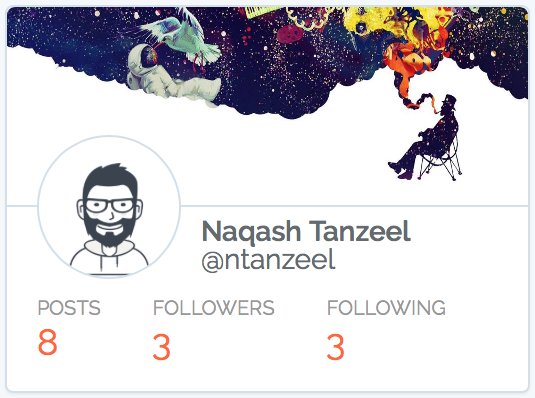
\includegraphics[width=1\textwidth]{Images/Design/UI/Widgets/Profile_Self}
		\caption{Self Profile}
		\label{fig:ProfileWidget_Self}
	\end{subfigure}
	\begin{subfigure}[b]{0.4\linewidth}
		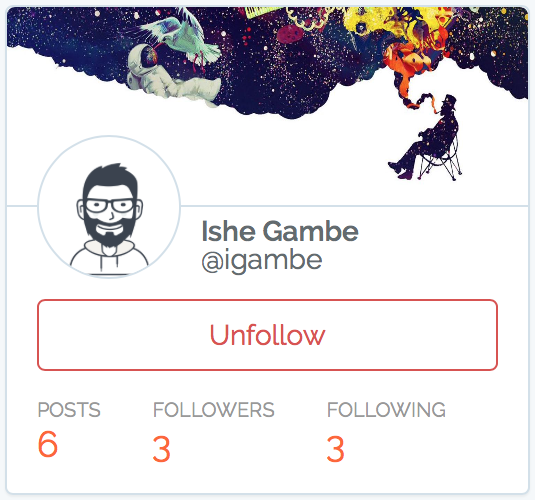
\includegraphics[width=1\textwidth]{Images/Design/UI/Widgets/Profile_Other}
		\caption{Others Profile}
		\label{fig:ProfileWidget_Other}
	\end{subfigure}
	\caption{The profile widget when display your own and someone else's profile.}
	\label{fig:ProfileWidget}
\end{figure}


\subsubsection{Trending} \label{sec:design-trending}
The widget shown in figure \ref{fig:trending} displays the top trending tags. The tags are displayed in descending order of how common they were in the last half an hour period. Each trending tag is then a link to the corresponding tag's feed in the discover page, allowing the user to find content relevant to that tag. The design of the widget is similar to the trending widget in Twitter (see figure \ref{fig:trending-twitter}), so that the user is familiar with the functionality it provides.

\begin{figure}[H]
	\centering
	\begin{subfigure}[b]{0.4\linewidth}
		
\includegraphics[width=1\textwidth]{Images/Design/trending-widget}
		\caption{Trending widget}
		\label{fig:trending}
	\end{subfigure}
	\begin{subfigure}[b]{0.4\linewidth}
		
\includegraphics[width=1\textwidth]{Images/Design/trending-twitter}
		\caption{Trending on Twitter}
		\label{fig:trending-twitter}
	\end{subfigure}
	\caption{Trending widget on Fidelis and Twitter.}
	\label{fig:TrendingWidgets}
\end{figure}

\subsubsection{Recommendations}
User recommendations that will be generated as discussed earlier in Chapter \ref{sec:ContentRecommendation} will need to be displayed to the user. Figure \ref{fig:RecommendationsWidgetDesign} shows the design for the user recommendations widget. The widget will show the user any new recommendations that have been generated for them, or old recommendations they have not interacted with. The widget will allow users to navigate to the profile of the recommendation, and will also have buttons which will enable the user to accept or reject the recommendations they have been provided with.

\begin{figure}[H]
\centering
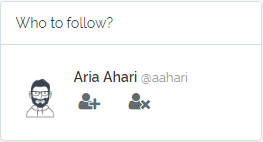
\includegraphics[height=1.5in]{Images/Design/RecommendationsWidgetDesign}
\caption{Design for the recommendations widget}
\label{fig:RecommendationsWidgetDesign}
\end{figure}

By providing recommendations as a widget, this will allow recommendations to be displayed to the user on multiple pages. With this in mind, the recommendations widget will appear for authorised users on the home, notifications and profile page.
